\documentclass[11pt]{article}

\usepackage[utf8]{inputenc}
\usepackage{amsmath, amssymb}
\usepackage{graphicx}
\usepackage[hidelinks]{hyperref}
\usepackage{geometry}
\usepackage{setspace}
\usepackage{titlesec}
\usepackage{booktabs}
\usepackage{tabularx}
\usepackage{caption}
\usepackage{csquotes}
\usepackage{float}
\usepackage{derivative}
\usepackage{subcaption}

\usepackage[
	style=nejm,
	citestyle=numeric-comp,
	sorting=none,
	doi=false,
	backend=bibtex]{biblatex}
\addbibresource{literature.bib}

% Geometry settings
\geometry{
	a4paper,
	total={6in, 9in},
	left=1.25in,
	top=1in,
}

% Title settings
\titleformat{\section}{\normalfont\Large\bfseries}{\thesection}{1em}{}
\titleformat{\subsection}{\normalfont\large\bfseries}{\thesubsection}{1em}{}

% Title
\title{An Experimental Analysis of the Influence of the Precision of Parameters in an Artificial Neural Network}
\author{Denise Katritschenko, Elias Reich, Sayed Abozar Sadat, Lukas Schwaiger\\
	\small University of Salzburg\\
	\small Department of Artificial Intelligence and Human Interfaces (AIHI) }

\date{\today}

\begin{document}

\maketitle

\begin{abstract}
	We study how the numerical precision of weights, activations, and gradients in neural networks can be reduced without sacrificing too much of the classification performance. Using MNIST as a dataset, we benchmark uniform 16–64-bit quantisation, mixed-precision formats, and post-training decimal rounding. The results reveal that (i) 16-bit end-to-end training preserves full accuracy for the MNIST dataset and the network used, (ii) three-decimal-place weight rounding while keeping 32-bit precision incurs minimal accuracy loss. These findings verify limits for memory- and energy-constrained usecases like inference in mobile devices.
\end{abstract}

\section{Introduction}
Artificial Neural Networks (ANNs) are a key part of today’s machine learning
systems. They’ve made huge progress in areas like image recognition, speech
processing, and self-driving cars. However, one of the biggest challenges with
ANNs is that they use a lot of memory and computing power. This becomes a
problem when you want to run them on devices with limited resources, such as
smartphones, embedded systems, or edge devices. \\ \\ To solve this,
researchers have looked into ways to make neural networks more efficient. A
common approach is to reduce the size of the network or shrink the input batch
size. But doing this can harm the network’s ability to learn and generalize. A
better strategy is to reduce the numerical precision of the network’s
parameters such as things like weights, activations, and gradients. This
method, called quantization, makes the model smaller and faster while using
less energy, without necessarily hurting accuracy. \\ \\ One advanced version
of this method is called mixed-precision quantization. Instead of using the
same number of bits for every layer in the network, mixed-precision assigns
different bitwidths depending on how important each part is. For example, the
early layers that handle low-level features might use higher precision, while
deeper layers could work fine with fewer bits. This flexible approach often
leads to better results than using a single fixed precision for the whole
model. Researchers have used a range of techniques, like gradient descent,
heuristics, and even evolutionary algorithms, to find the best bitwidth
settings for each layer. \\ \\ Another method that helps reduce resource usage
is network pruning. This means cutting out parts of the network that don’t
contribute much to its performance. One interesting way to do this is with
simulated annealing, a search algorithm that mimics the process of cooling
metal to find a stable structure. It doesn’t need gradient information and can
still find good network shapes by exploring many possibilities. This makes it
useful when you want to shrink a network without going through heavy
retraining. \\ \\ Previous studies have shown that reducing the precision of
neural network parameters can lead to significant improvements in memory usage
and processing speed. Even when precision is reduced to very low levels, models
can still perform competitively on complex tasks. However, while these early
results are promising, the overall effects of lowering precision, especially
how it influences model accuracy, training behavior, and storage efficiency,
are still not fully understood and deserve more detailed investigation. \\ \\
This is where our experimental work begins. In this paper, we take a closer
look at how different levels of parameter precision affect the behavior and
performance of neural networks. Our goal is to understand what happens when we
reduce precision in various ways, and how much we can lower it before
performance starts to drop. \\ \\ We start by testing how reducing precision
during both training and inference affects model accuracy and runtime. Next, we
look at what happens when we train the network using full precision, but lower
the precision only during inference. This setup is common in real-world
applications, where a powerful machine handles training, but the final model is
deployed on a lightweight device. Then, we run a series of tests where we round
the trained weights to a limited number of decimal places. This helps us see
how much we can simplify the stored weight values without hurting accuracy too
much. This is especially useful for devices with very limited storage. We also
try out mixed-precision training, using a mix of FP16 and FP32 formats. On top
of that, we experiment with different types of gradient clipping, like global
norm clipping and value clipping, to see how they affect training stability and
final accuracy. Even though we use relatively simple network architectures and
datasets, our results show that neural networks are quite robust to
low-precision settings. In some cases, we were able to round weights to just
three decimal digits and still get nearly the same accuracy as the
full-precision version. These findings show that it’s possible to significantly
reduce the memory and compute needs of neural networks without losing much
performance. This makes them more practical for use in low-resource settings.
It also opens the door for more advanced techniques that combine quantization,
pruning, and precision-aware training to build highly efficient models for
real-world applications.

\section{Background}

A typical neuron in a neural network performs a weighted sum of its inputs,
followed by an activation function:
\[
	a = \omega^\top x + b,\quad \hat{y} = \sigma(a),
\]
where \( \omega \in \mathbb{R}^n \) is the weight vector, \( b \in \mathbb{R}
\) is the bias, \( x \in \mathbb{R}^n \) is the input, and \( \sigma \) is a
nonlinear activation function (e.g., sigmoid or ReLU).

Training is conducted via backpropagation, where gradients of a loss function
\( L(\hat{y}, y) \) with respect to the model parameters are computed. For
example, using the mean squared error:
% \[
% L(\hat{y}, y) = (\hat{y} - y)^2, \qquad \pdv{L}{\omega_i} = 2(\hat{y} - y) \cdot \odv{\sigma}{a} \cdot x_i.
% \]

\begin{align*}
	L(f(x_1, x_2)) & = {(\sigma(\omega^T x + b) - y)}^2 \\
	               & = {(\sigma(a) - y)}^2              \\
	               & = {(\hat y - y)}^2
\end{align*}
\begin{alignat*}{3}
	\pdv{L}{\omega_1} & = \pdv{L}{\sigma} &  & \pdv{\sigma}{a}      &  & \pdv{a}{\omega_1} \\
	                  & = 2(\hat y - y)~~ &  & \odv{}{a}\sigma(a)~~ &  & x_1
\end{alignat*}

Memory and computational requirements during training are substantial, as
gradients, activations, and parameters must be stored and updated iteratively.
In contrast, inference requires only a forward pass, making it more amenable to
optimization via precision reduction.

\section{Memory Efficiency and Numerical Formats}

To reduce memory usage and computational load, precision-aware techniques such
as quantization and mixed-precision training are increasingly employed. Instead
of using 32-bit or 64-bit floating-point formats, parameters can be stored in
16-bit or even 8-bit fixed-point representations.
Figure~\ref{fig:floatingPointFormat} depicts the general floating point format
and terminology of significand, base, and exponent.
Tables~\ref{tab:binary-bits} and~\ref{tab:binary-precision} provide an overview
of the different floating point types and their respective characteristics.

\begin{figure}[H]
	\centering
	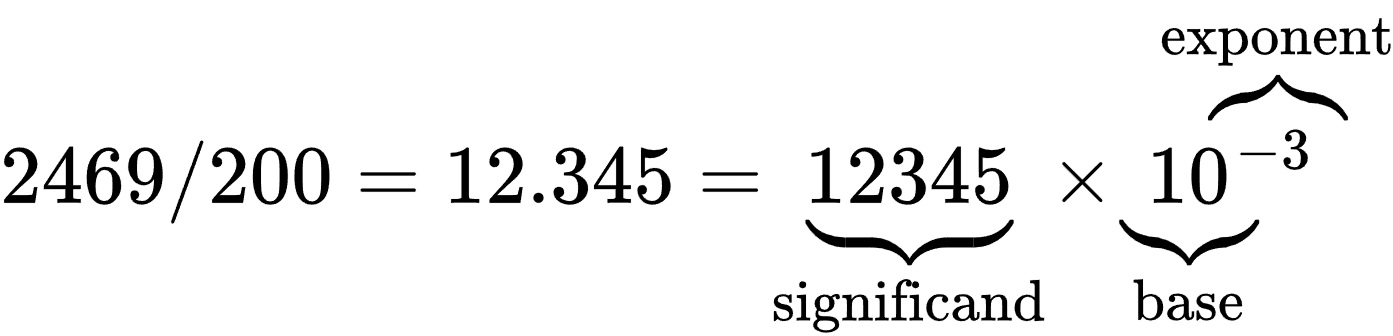
\includegraphics[width=0.8\textwidth]{figures/float.png}
	\caption{Illustration of standard floating-point format.}\label{fig:floatingPointFormat}
\end{figure}

\begin{table}[H]
	\centering
	\begin{tabular}{@{}lcccc@{}}
		\toprule
		\textbf{Type} & Sign & Exponent & Significand & Total \\
		\midrule
		Half  (FP16)  & 1    & 5        & 10          & 16    \\
		Single (FP32) & 1    & 8        & 23          & 32    \\
		Double (FP64) & 1    & 11       & 52          & 64    \\
		\bottomrule
	\end{tabular}
	\caption{Field widths (in bits) of common IEEE754 formats (adapted from~\cite{fparithmetic}).}\label{tab:binary-bits}
\end{table}

\begin{table}[H]
	\centering
	\begin{tabular}{@{}lccc@{}}
		\toprule
		\textbf{Type} & Exponent bias & Precision (bits) & Decimal digits \\
		\midrule
		Half  (FP16)  & 15            & 11               & $\sim$3.3      \\
		Single (FP32) & 127           & 24               & $\sim$7.2      \\
		Double (FP64) & 1023          & 53               & $\sim$15.9     \\
		\bottomrule
	\end{tabular}
	\caption{Range and precision characteristics of the same formats (adapted from~\cite{fparithmetic}).}\label{tab:binary-precision}
\end{table}

\section{Related Work}

Prior research in this domain can be broadly classified into two categories:

\subsection*{Quantization During Training}
Several studies have explored training neural networks with reduced precision
directly. Notable contributions include:
\begin{itemize}
	\item \textbf{Mixed Precision Training}, which leverages float16 arithmetic for speed while maintaining float32 master weights~\cite{micikevicius2017mixed}.
	\item \textbf{DoReFa-Net}, which quantizes weights, activations, and gradients to arbitrary bitwidths~\cite{zhou2018dorefa}.
	\item \textbf{Q-BERT}, a quantized BERT model that maintains accuracy using only 4-bit weights~\cite{shen2020qbert}.
\end{itemize}

\subsection*{Post-Training Quantization}
Other approaches focus on converting pretrained models into lower-precision
equivalents:
\begin{itemize}
	\item \textbf{Integer-Only Quantization} using symmetric quantization scales~\cite{jacob2018quantization}.
	\item \textbf{GPTQ}, a method for quantizing large transformer models without retraining~\cite{frantar2022gptq}.
	\item \textbf{SmoothQuant}, which scales activations to better match weight ranges during quantization~\cite{xiao2024smoothquant}.
\end{itemize}

\section{Experimental Design}

We trained a simple fully connected neural network on the MNIST dataset,
consisting of 60,000 training and 10,000 test grayscale images of handwritten
digits (28×28 pixels, see figure~\ref{fig:mnistSample}). Model training was
performed under varying parameter bitwidths, and 5-fold cross-validation to
evaluate the model performance. The structure of the MLP is depicted in
figure~\ref{fig:mlpStructure}.

\begin{figure}[H]
	\centering
	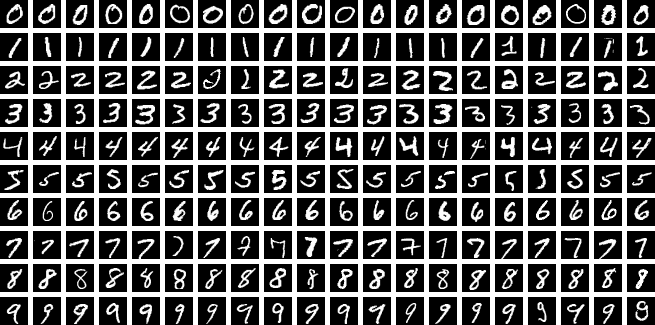
\includegraphics[width=0.85\textwidth]{figures/mnist.png}
	\caption{Sample images from the MNIST dataset.}\label{fig:mnistSample}
\end{figure}

\begin{figure}[H]
	\centering
	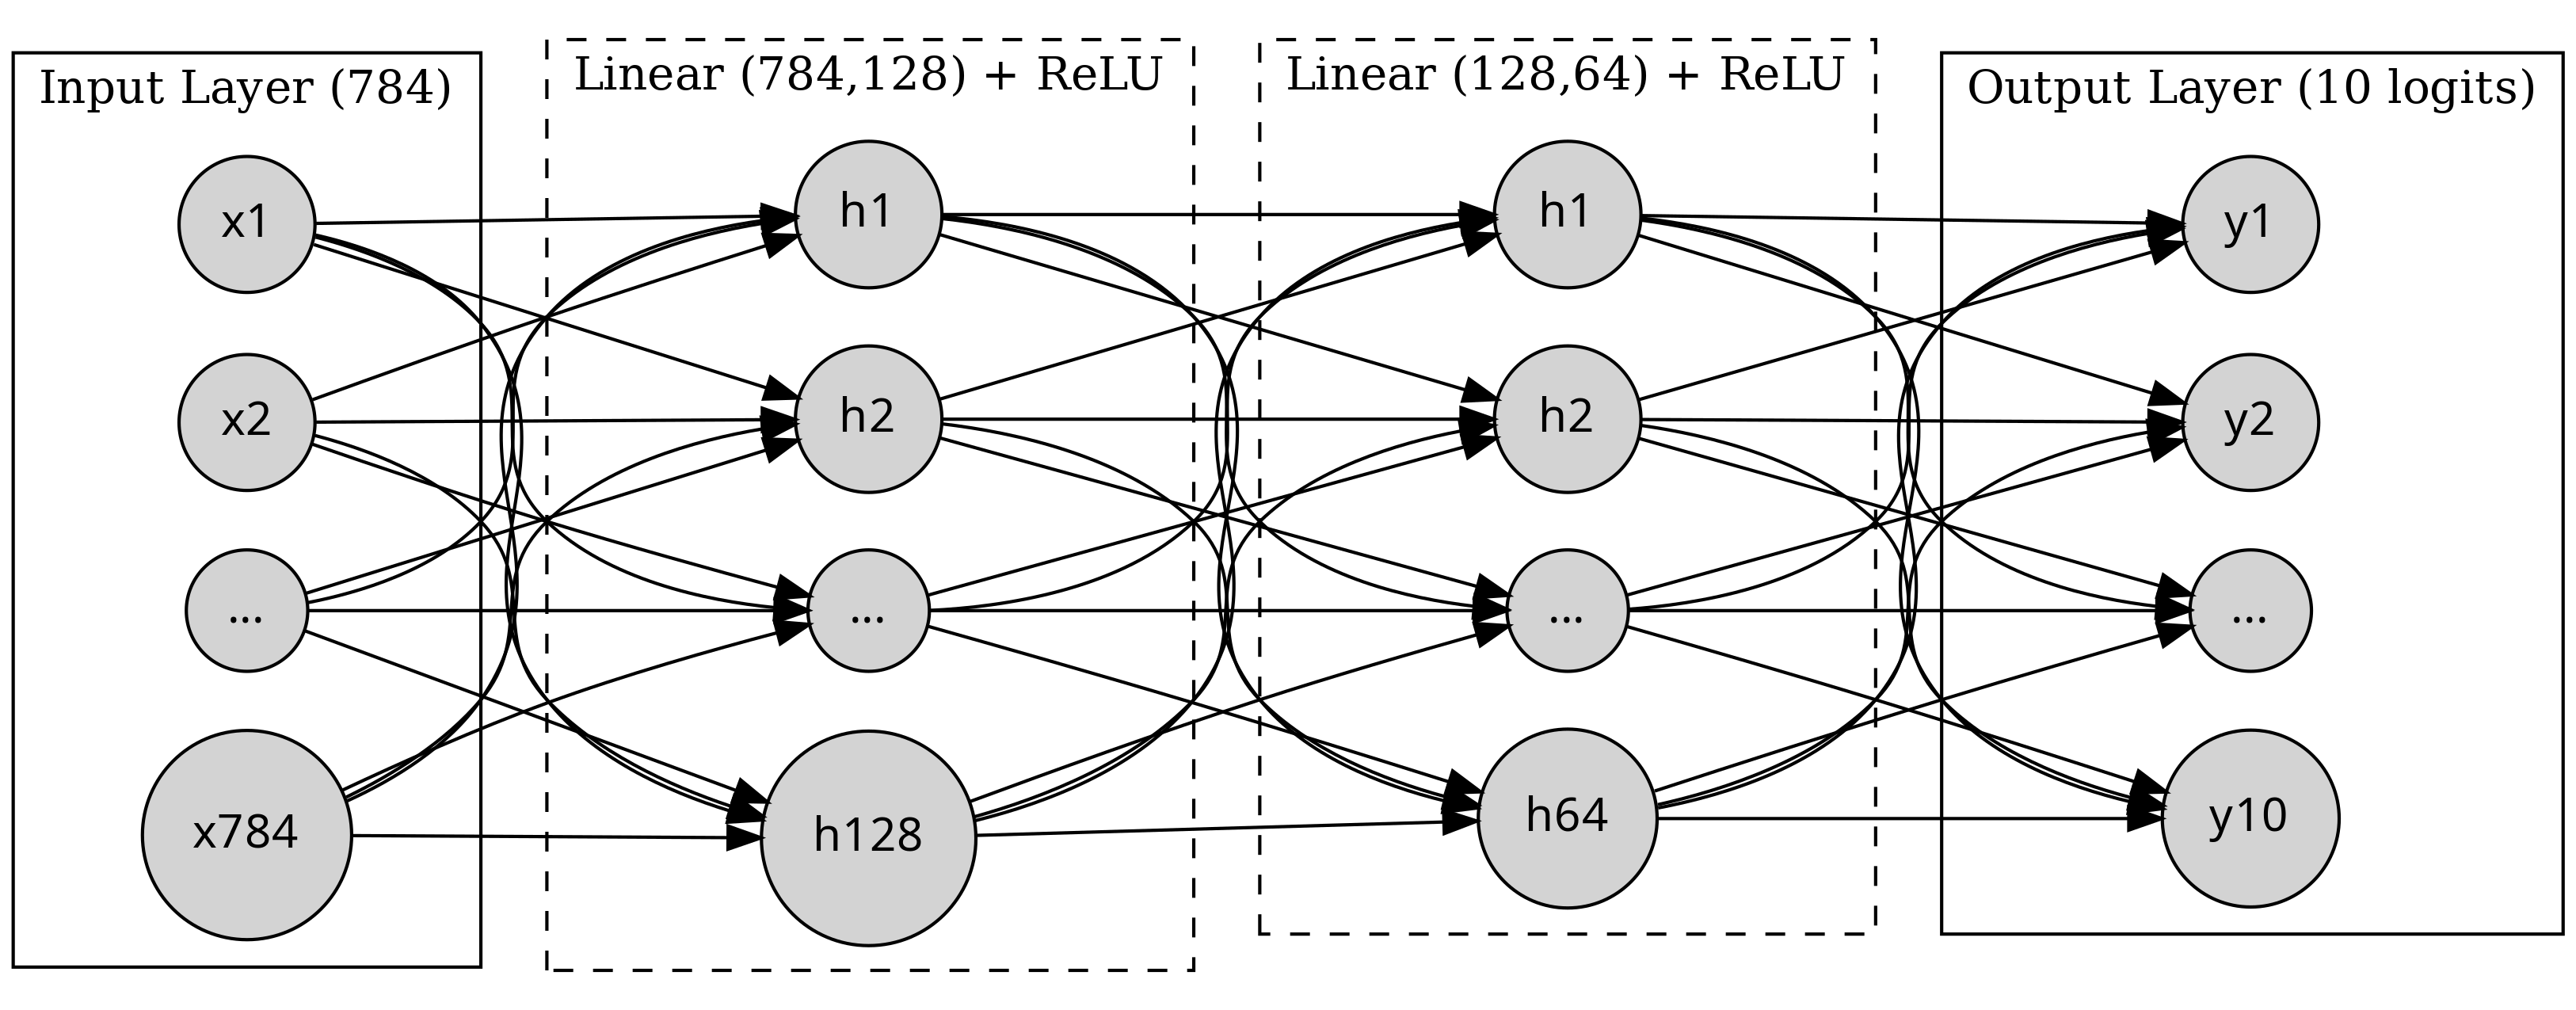
\includegraphics[width=0.85\textwidth]{figures/mlpStruc.png}
	\caption{MLP structure used in the experiments.}\label{fig:mlpStructure}
\end{figure}

\section{Results}
In the first experiment, every floating-point tensor that is used inside the
training loop was converted to a lower precision data type. This therefore
includes the weights and biases, activations, gradients, optimizer states, etc.
The types tried were float64, float32, and float16.

\subsection*{Accuracy Across Bitwidths}
Figure~\ref{fig:modelAccTrainAndInf} shows how the accuracy changed after the
models were trained on the different precision settings. Keep in mind that the
y-axis is not starting from zero, so the absolute height differences are
amplified visually, though the delta is only around $.1$ percent. Re-training
the models and re-evaluating them has also lead to the accuracies being
``reversed'', meaning the float64 model had the least accuracy. It is safe to
assume that the model accuracy has neither decreased, nor increased.
\begin{figure}[H]
	\centering
	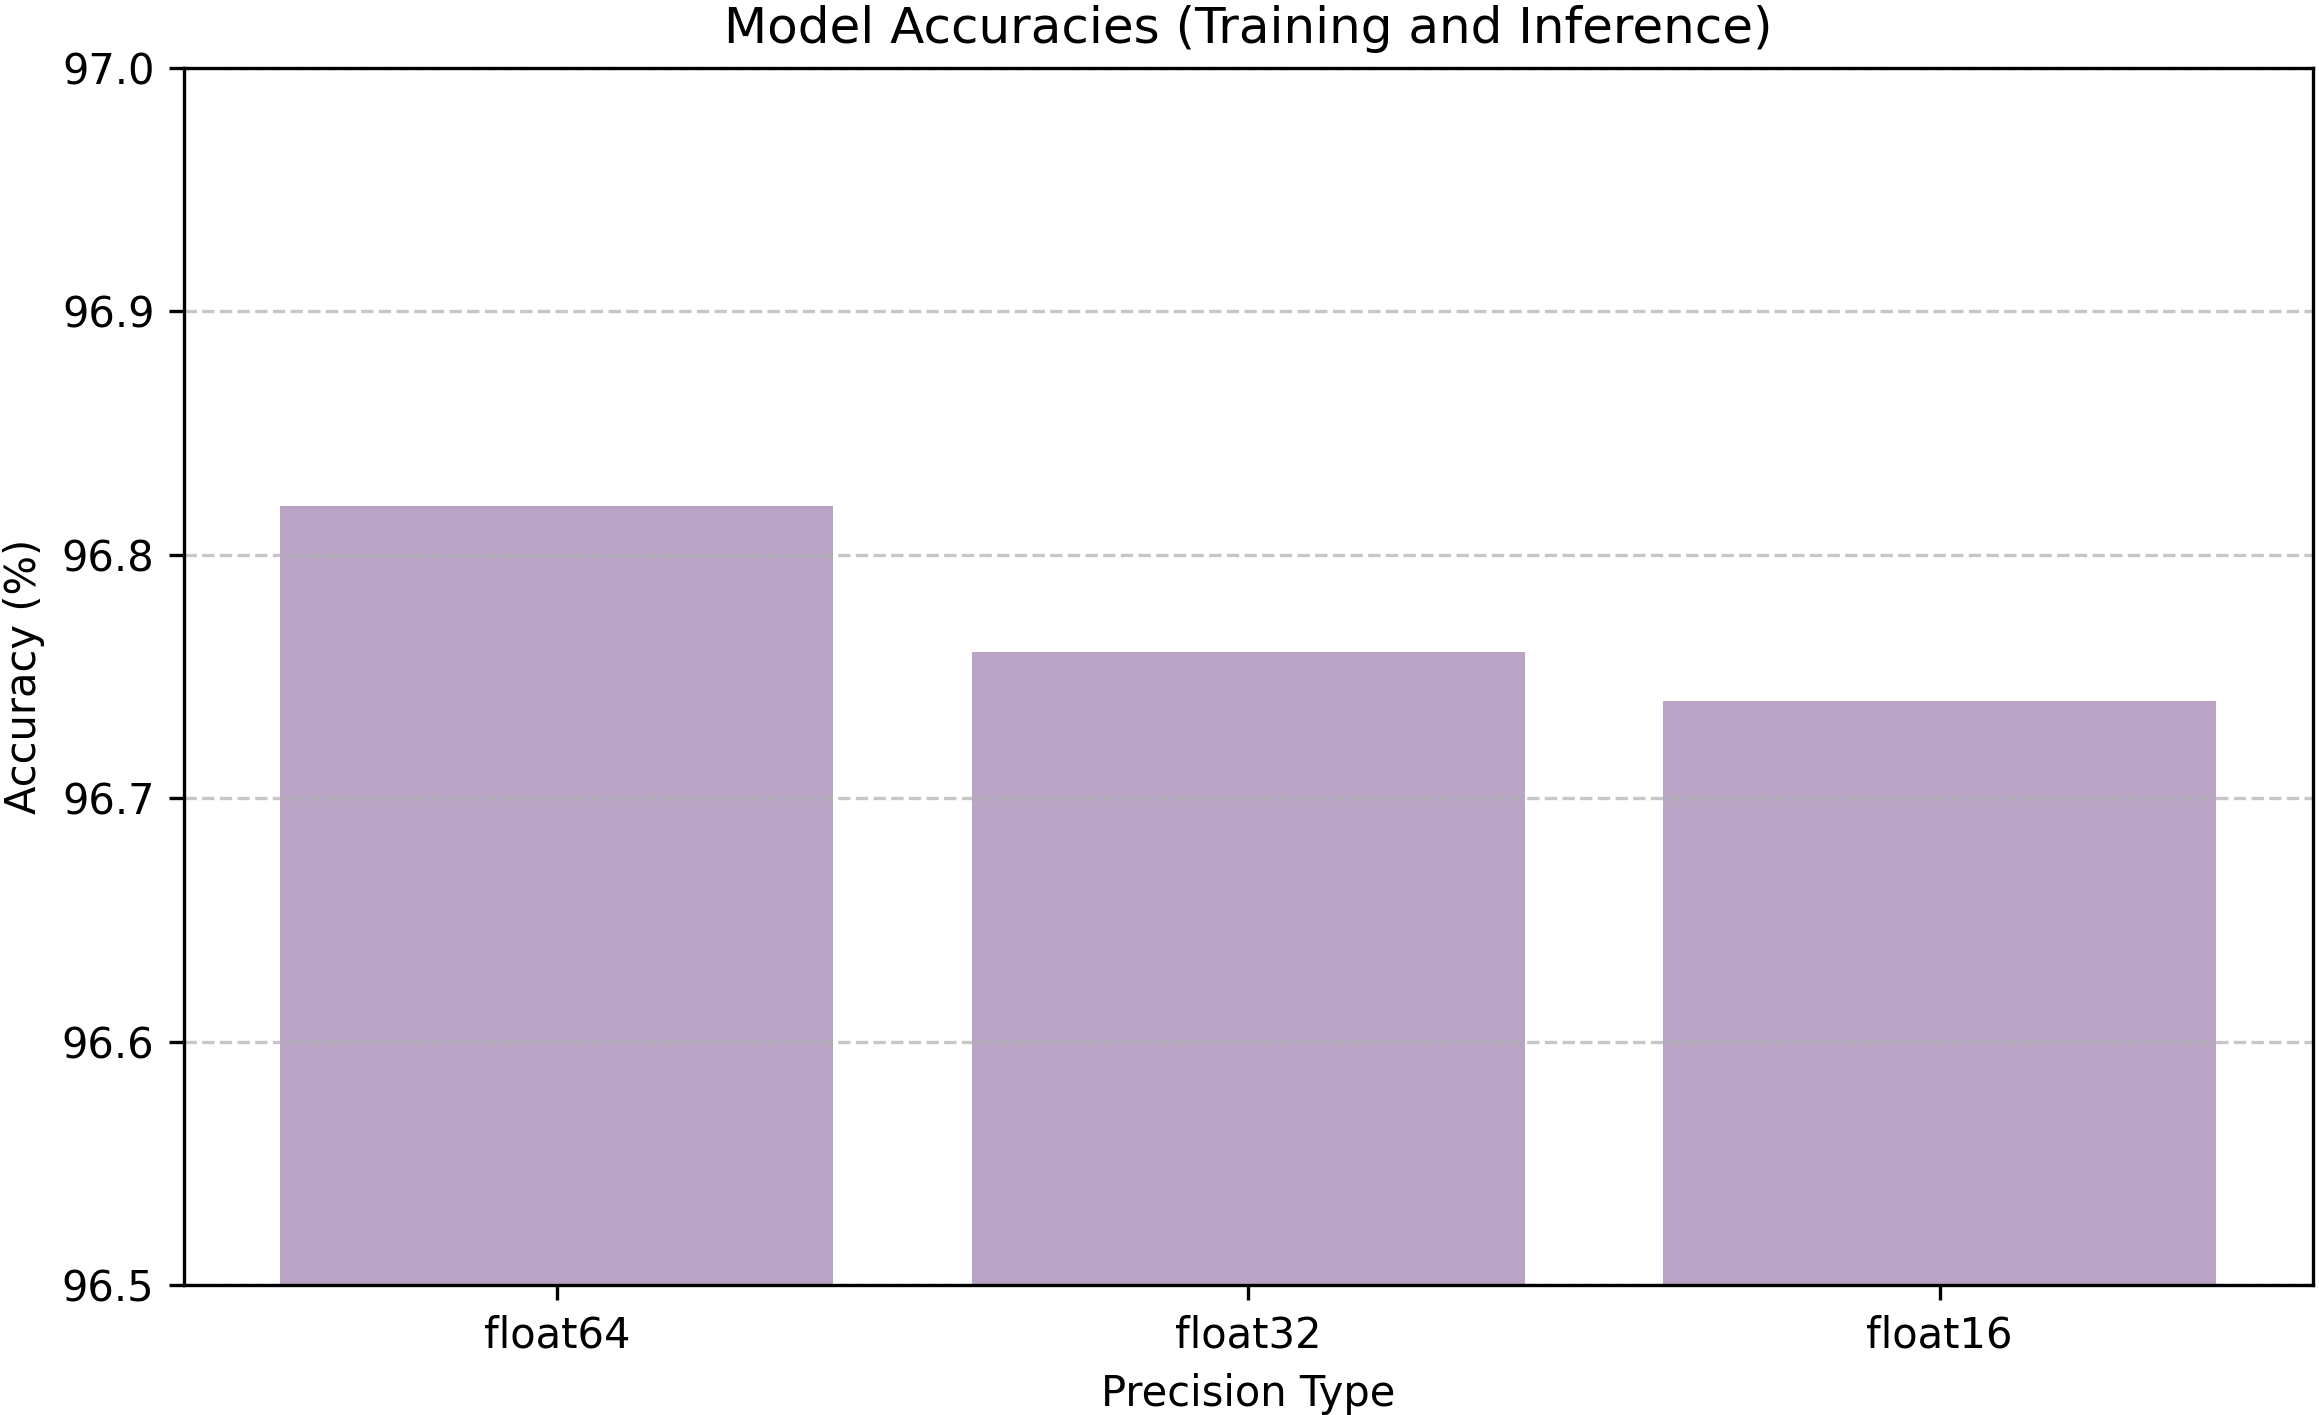
\includegraphics[width=0.85\textwidth]{figures/trainingAndInference.png}
	\caption{Model accuracy evaluated after training with the different precisions.}\label{fig:modelAccTrainAndInf}
\end{figure}

\subsection*{Training and Inference Time}
Also analyzed were the times needed for both the training and inference.
Figure~\ref{fig:modelEvalTrainTimes} depicts the times measured in the training
loop and later on at the inference stage. Again, the times are almost identical
in both regards, and neither a real speed-up nor a slow-down has been measured.
\begin{figure}[H]
	\centering
	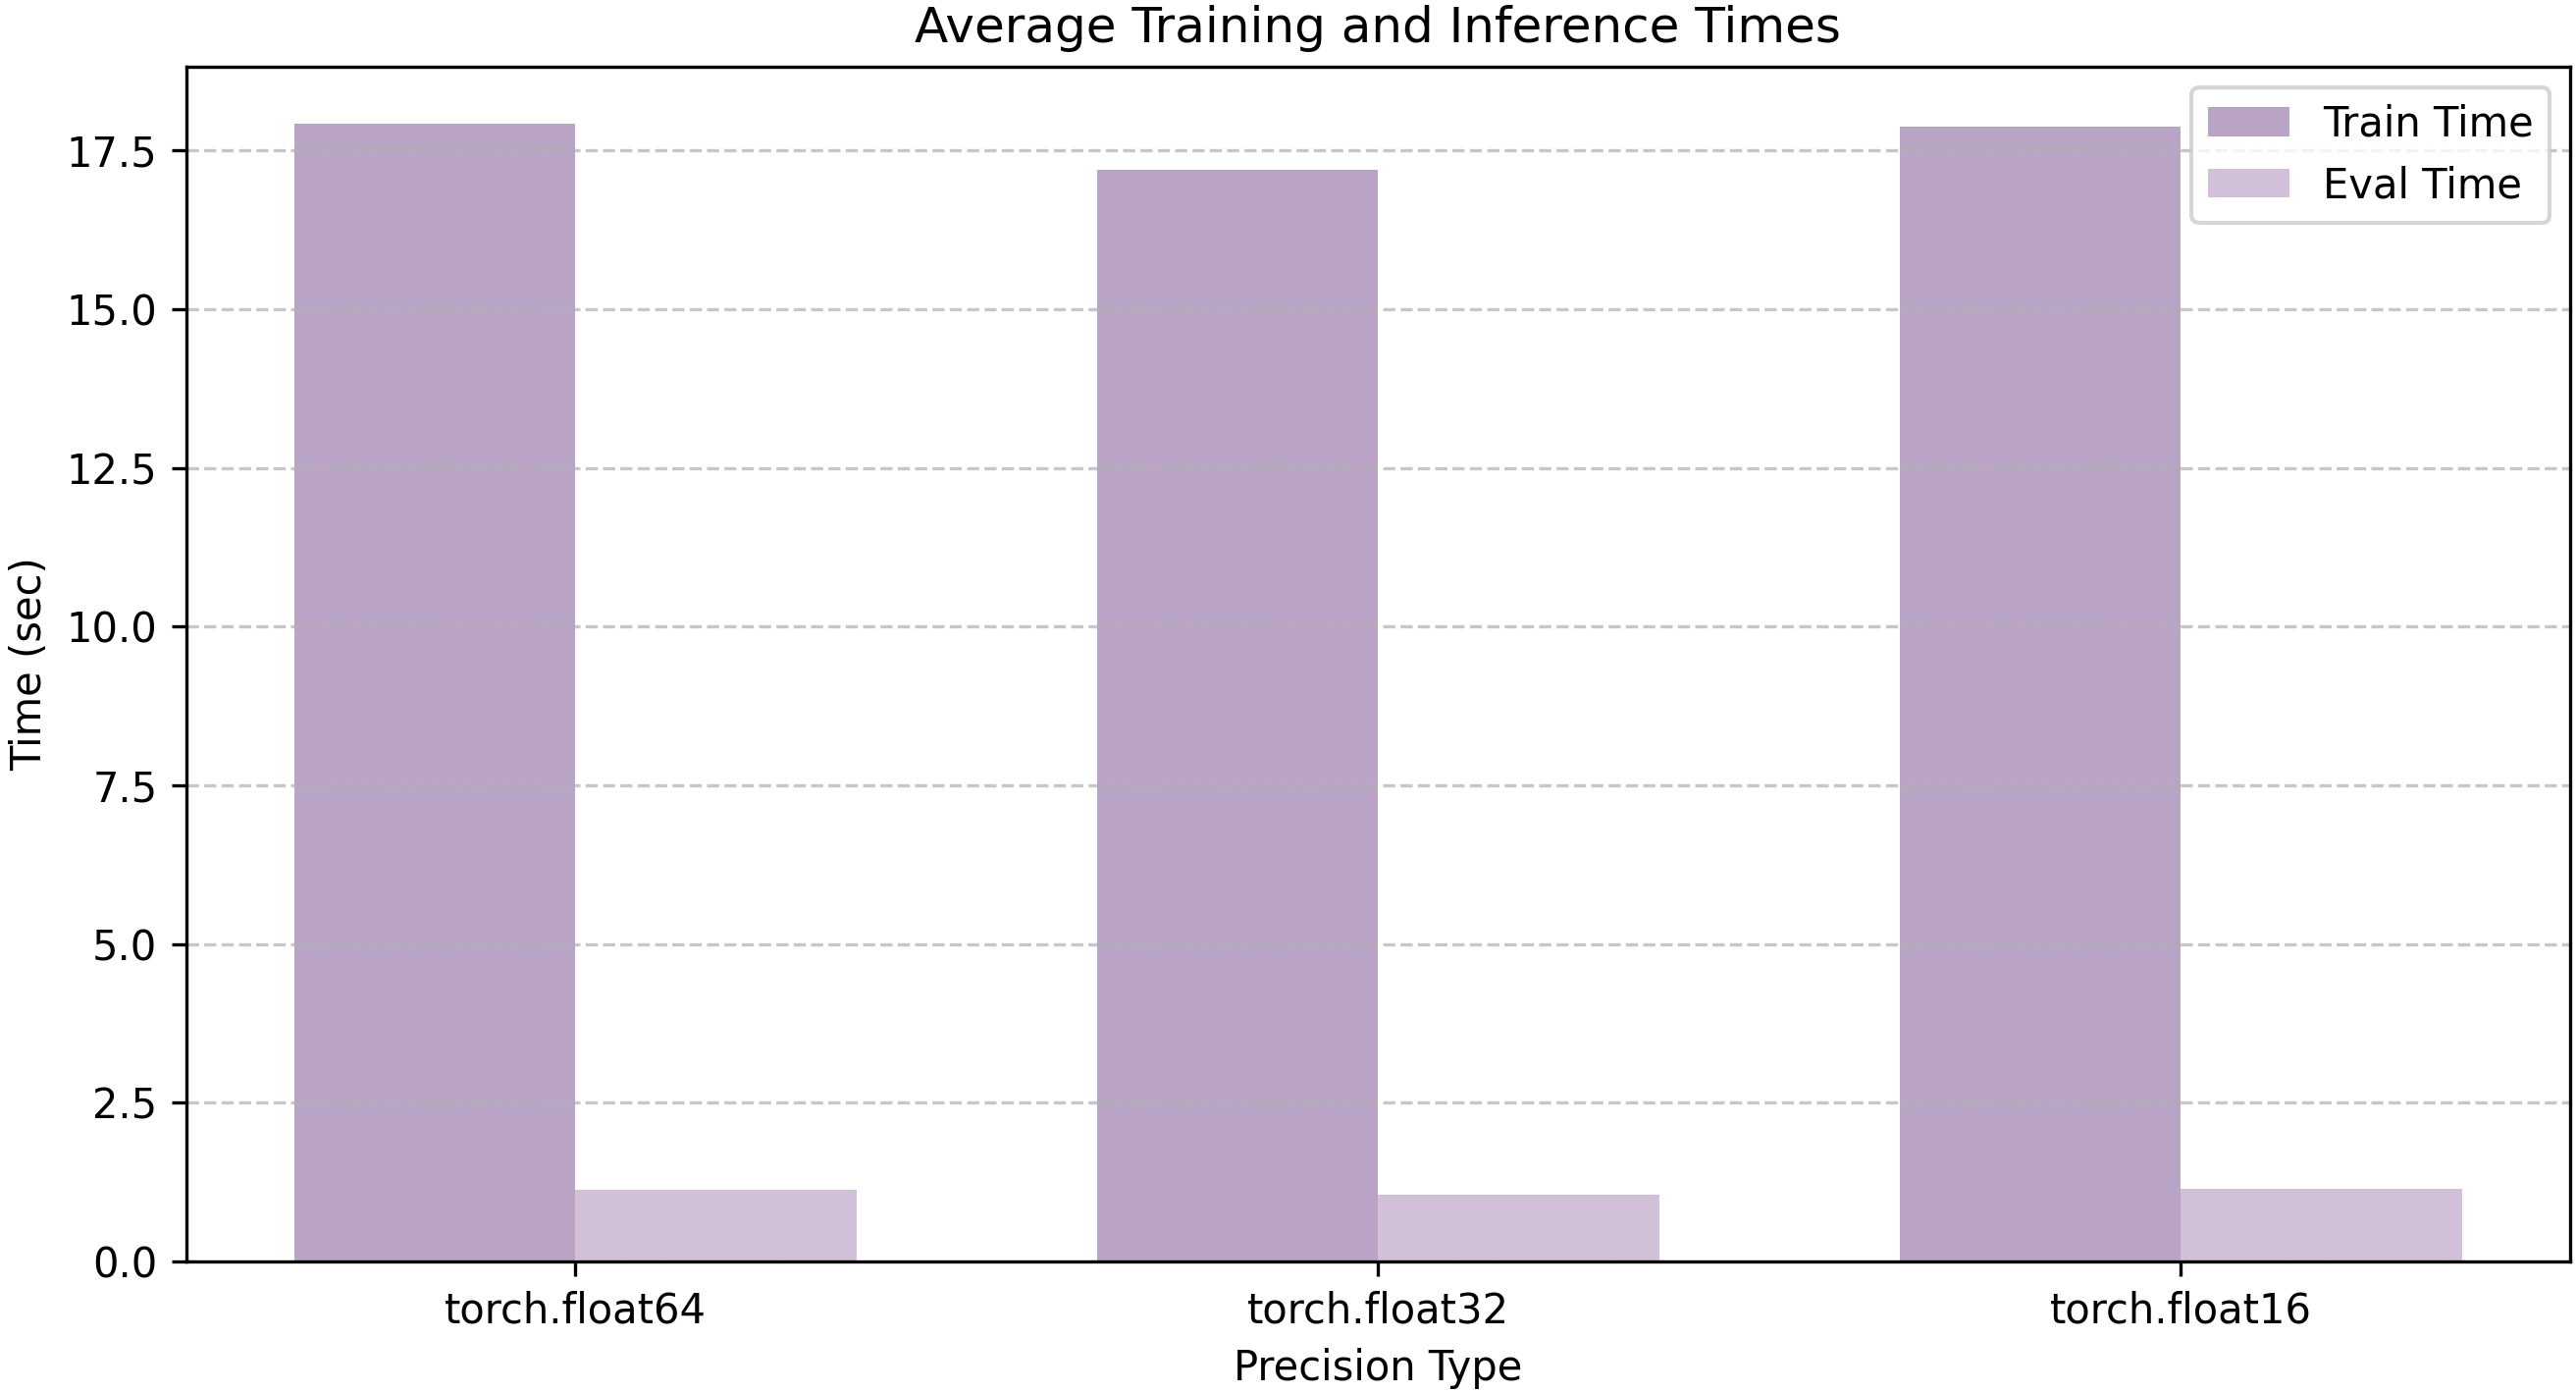
\includegraphics[width=0.85\textwidth]{figures/times.png}
	\caption{Training and evaluation times for the different precisions.}\label{fig:modelEvalTrainTimes}
\end{figure}

\subsection*{Inference-Only Testing}
This third experiment was conducted to test a possible post-training precision
reduction. For this, the model was trained on the highest precision (float64)
and then quantized at the inference stage.
Figure~\ref{fig:inferenceOnlyTesting} shows that the accuracy of the baseline
(float64 training AND inference) is maintained as the precision is decreased at
the later stages. In contrast to the \textit{Accuracy Across Bitwidths}
experiment, there are no fluctuations at all because for the lower precisions,
there was no new model trained.
\begin{figure}[H]
	\centering
	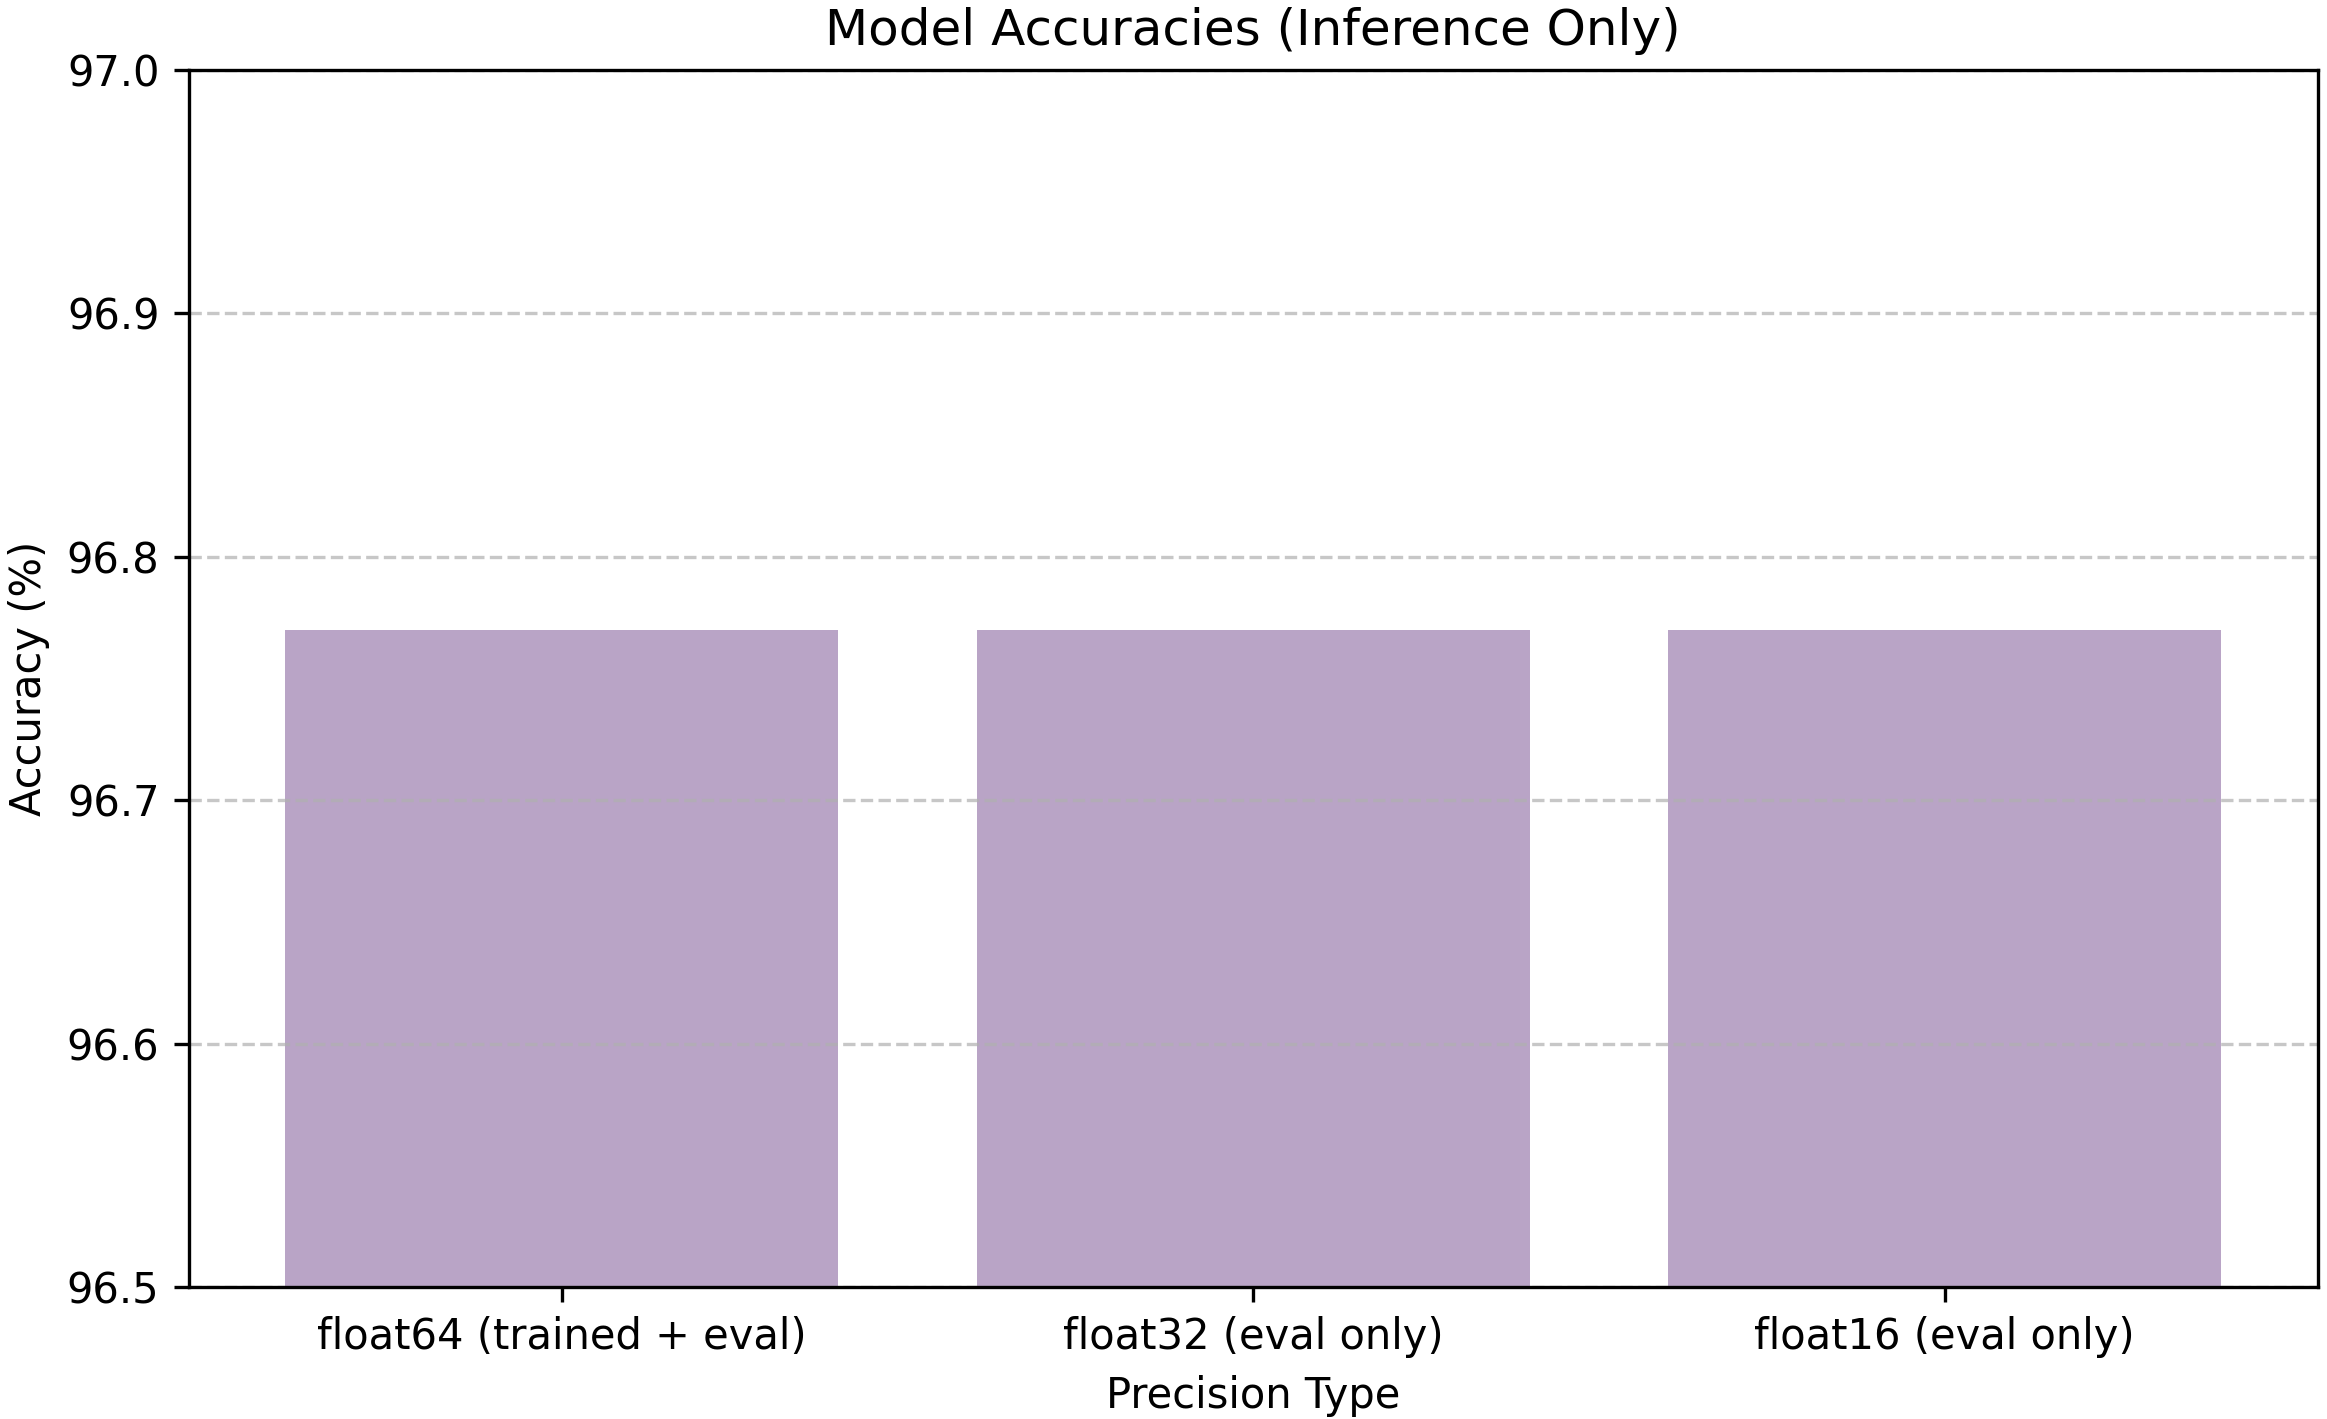
\includegraphics[width=0.85\textwidth]{figures/inferenceOnly.png}
	\caption{Inference accuracy using float64-trained weights followed by quantization.}\label{fig:inferenceOnlyTesting}
\end{figure}

\subsection*{Automatic Mixed Precision and Gradient Clipping}
As a next experiment, \dots %Sayed, also use the other images?
\begin{figure}[H]
	\centering
	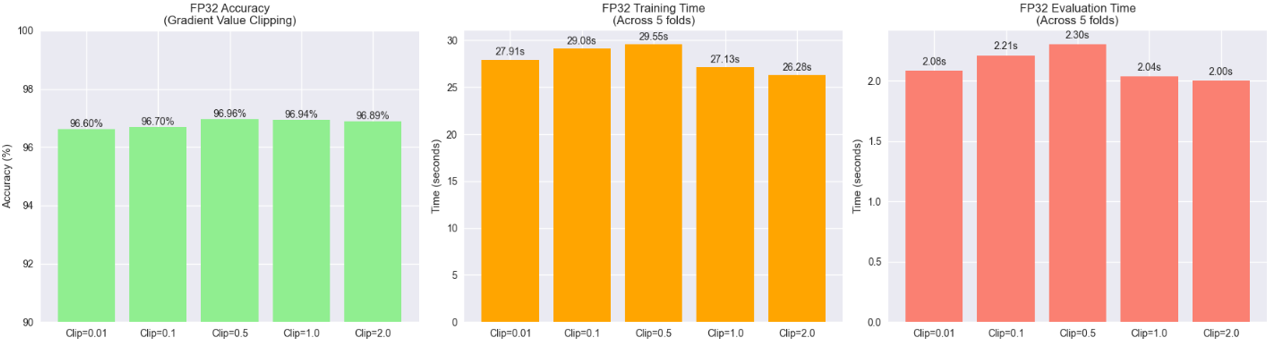
\includegraphics[width=0.85\textwidth]{figures/gradclip_32.png}
	\caption{Inference accuracy using float32-trained weights with AMP and gradient clipping.}
\end{figure}

\subsection*{Effect of Decimal Rounding}

A non training related issue is the storage of the NN parameters. Usually, the parameters
are stored in the format that was chosen to train with. This is best for reproducibility
as well as accuracy when doing inference with the trained model weights. The datatype  
precision has a higher impact during training though, which begs the question if one could
omit precision from the model weights. In this section, we explore a naive quantization
method: Rounding to a fixed number of decimals. With significantly little decimals and a
reasonable range for the integer part, one could store only the significant and provide
base as well as exponent as metadata. When loading the model, the weights are converted
back to floating point, with whatever precision is desired. Only the weights are quantized;
the input data, as well are the values propagated through the network are at full
precision.

The first step is to examine the distribution of parameter values. By the standard
deviation around modes one can make an educated guess as to how many decimals are needed.
The range will decide how large the integer part may get. Reading from the 
distribution is just a heuristic though, so we will also test the hypotheses.


\begin{figure}[H]
	\centering
	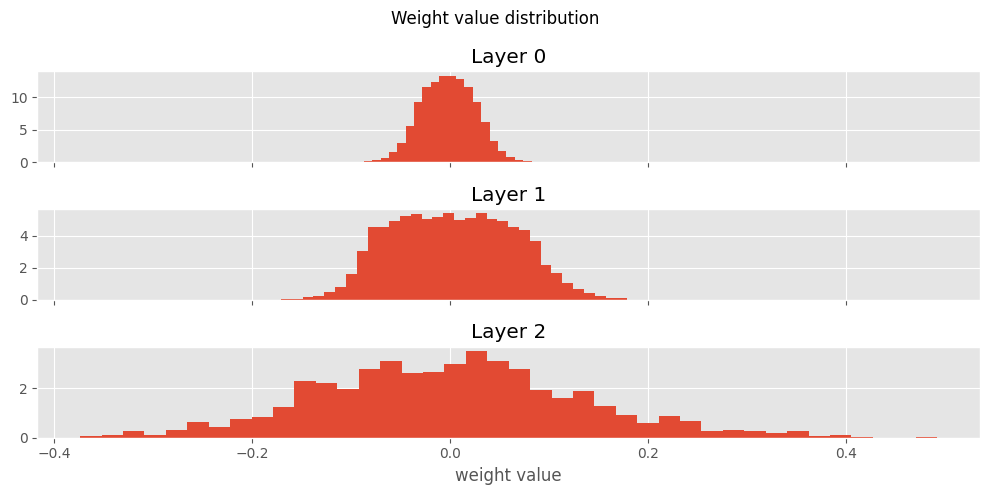
\includegraphics[width=0.85\textwidth]{figures/118_dist.png}
	\caption{
		Distribution of model weights in each layer. The values are in $[-0.5, 0.5]$,
		this means no integer part is needed in this example. Generally, with normalized data
		and the quite popular L1-/L2-/Batch-Norm layers, weight values in $[-1, 1]$ is to be expected.}
\end{figure}

\begin{figure}[H]
	\centering
	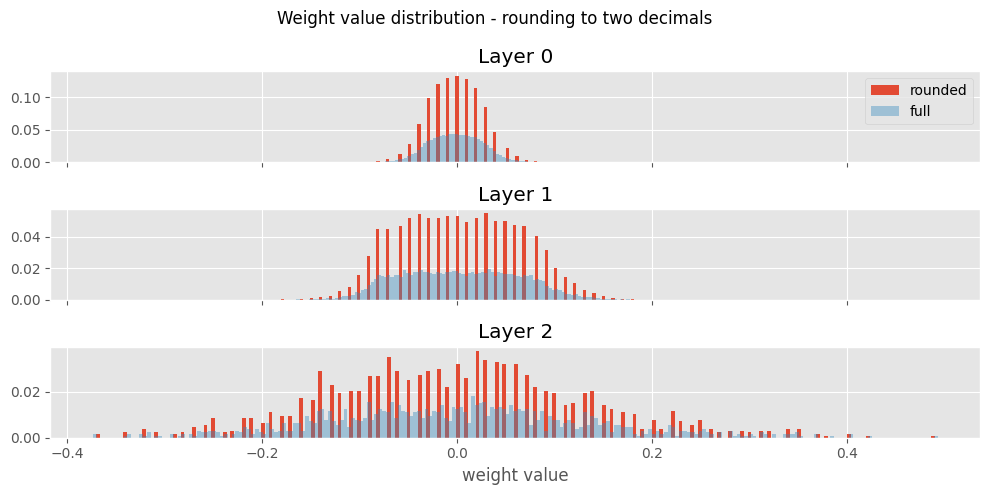
\includegraphics[width=0.85\textwidth]{figures/118_dist2.png}
	\caption{Distribution of model weights in each layer after rounding to two decimals.
	This appears to be a good approximation already.}
	\label{fig:118_2}
\end{figure}

\begin{figure}[H]
	\centering
	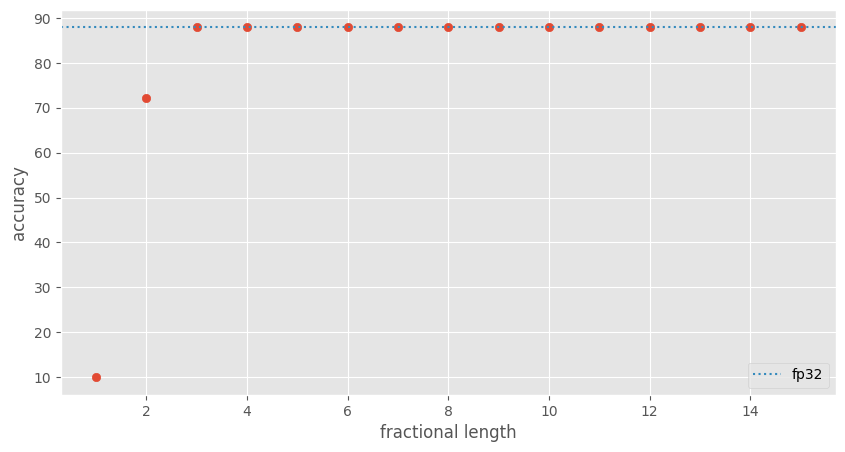
\includegraphics[width=0.85\textwidth]{figures/118_accuracy.png}
	\caption{Test Accuracy vs.\ number of decimal digits retained in weights.}
	\label{fig:118_acc}
\end{figure}

Figure~\ref{fig:118_acc} shows how rounding the decimal part affects the test accuracy.
For just one decimal the model has a maximum of 19 different weights at its disposal,
which makes the model have only 10\% accuracy, random guessing with a 10 class problem.
Two decimals perform significantly better. At 70\% accuracy the model gets close to the
full precision 88\% accuracy with 32 bit floating point. Making and educated guess on
distribution such as Figure~\ref{fig:118_2} seems to be a good heuristic for this example.
At just 3 decimals, the full 32 bit precision is reached. Thus we can conclude that with
just 10 bit for representing 3 decimals, no bits for the integer part and one additional
bit for the sign, only 11 bit must be stored to have the best performing model for
inference.


\section{Summary}
\begin{itemize}
	\item \textbf{16-bit is enough for this classification task}: End-to-end float16 preserved the accuracy.
	\item \textbf{Three decimals suffice}: Storing weights down to fractional length $3$ caused no visible accuracy loss.
\end{itemize}

\section{Discussion}

The results of the first experiments have shown that either the selected task
(MNIST classification) was not complex enough to be affected by the decrease in
accuracy, or the accuracy would need to be decreased even further than float16.

Otherwise, the results generally indicate that networks trained and evaluated
with as low as 16-bit precision can achieve comparable performance to their
high-precision counterparts. Moreover, rounding pretrained weights to just 3
decimal digits preserves full accuracy, opening the door to aggressive
post-training quantization.

This is particularly relevant for edge devices and real-time applications where
memory and compute constraints are more relevant.

\section{Conclusion and Future Directions}

This work confirms that for relatively simple tasks like MNIST classification,
significant reductions in parameter precision can be achieved without
compromising performance. Our future efforts will extend this analysis to more
complex datasets (e.g., CIFAR-10, ImageNet) and deeper architectures, and
explore advanced quantization-aware training techniques.

\newpage
\printbibliography%
\end{document}
